
\section{Hall effect}

The Hall effect is a consequence of the Lorentz force on a moving charge. To first understand this

\TODO{Introduction to Boltzman transport theory?}




As an electron (hole) moves along a rectangular slab subject to a perpendicular magnetic field, the electrons (holes) are deflected to one side of the slab. Eventually the charge density one one side becomes high enough that the Coulomb repulsion force of the density on subsequent charge carriers balances the Lorentz force and an equilibrium voltage between either side of the slab is reached. This voltage is known as the Hall voltage, $V_H$ and is given by,
\begin{equation}
    V_H = -\frac{IB_{\perp}}{ned}
\end{equation}
where $I$ and $B_{\perp}$ are the current and perpendicular magnetic field and $n$, $e$ and $d$ are the carrier density, charge and slab thickness respectively. $V_H$ is what is measured in our experiment. This is usually further abstracted to the Hall coefficient, $R_H$, which encapsulates the carrier density for a metal as follows,
\begin{equation}
    R_H = \frac{V_H d}{IB_\perp} = \frac{1}{ne}
\end{equation}

% \subsection{Temperature dependent effect of band structure}
% 
% Although there is not an explicit temperature dependent term in the Hall relation above, certain band structure features may affect the carrier density as a function of temperature. Perhaps the best known is that of a region of flat, high \ac{DOS}, band structure close to the Fermi energy which can only be accessed by carriers when the thermal energy is high enough. As described in section~\ref{Sec:Intro:PropertiesBSCO}, there is such a feature in the band structure in the overdoped portion of \ac{BSCO} and many other cuprates.

\subsection{Effects of Fermi surface topology}

Ostensibly, a hole-like Fermi surface would be expected to demonstrate positive Hall coefficient and an electron-like Fermi surface a negative, however it is possible to obtain the exact opposite due to the curvature of the Fermi surface~\cite{Narduzzo2008}. 

For a 2D metal in the weak field semiclassical limit, Ong determined that the transverse conductivity, $\sigma_{xy}$ from which $R_H$ is derived can be obtained by integrating the mean free path vector, $\vect{l_k} = \vect{v_k}\tau_k$ over the Fermi surface ($\vect{v_k}$ is the Fermi velocity and $\tau_k$ is the momentum dependent scattering rate). This is illustrated in figure~\ref{Fig:Theo:NegativeCurvatureLSCO} which integrates over a Fermi surface with a long mean free path in the $(\pi, \pi)$ direction and shows how the resulting $\vect{l_k}$ traces two loops in opposite directions giving rise to a larger `negative' loop from the negative curvature even though the overall surface has a positive curvature.
\begin{figure}[htbp]
    \begin{center}
        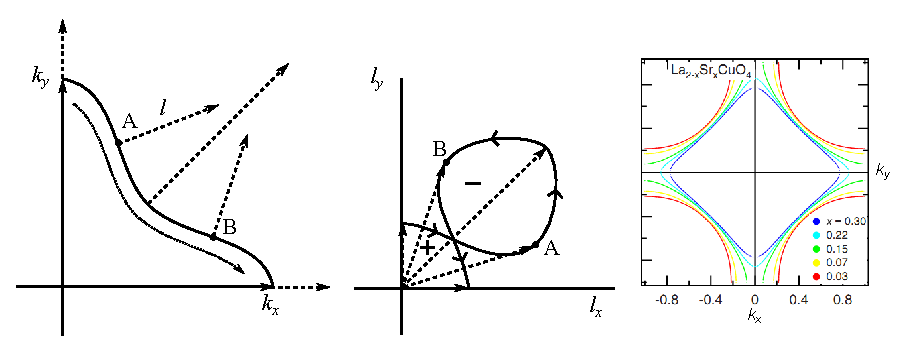
\includegraphics[scale=0.9]{Chapter-Theory/Figures/NegativeCurvatureLSCO/NegativeCurvatureLSCO}
        \caption{Left illustrates a negatively curved Fermi surface with a long mean free path along the $k = (\pi, \pi)$ portion and the integral progressing along the dotted line. Middle shows how the mean free path vector changes along the integral line tracing two loops of opposite direction. Adapted from ref.~\cite{Narduzzo2008}. Right shows the progression of the \ac{BSCO} Fermi surface about the van-Hove singularity. Adapted from ref.~\cite{Kondo2004}.}
        \label{Fig:Theo:NegativeCurvatureLSCO}
    \end{center}
\end{figure}
This illustrated scenario is close to what we find in the cuprates at high doping. Here the mean free path is affected by the anisotropic scattering rate detailed in the introduction section and the proximity of the van-Hove singularity leads to negative curvature in the long flat sides of the Fermi surface as it changes between hole-like and electron-like, as shown for \ac{BSCO} in the right side panel of figure~\ref{Fig:Theo:NegativeCurvatureLSCO}, adapted from ref~\cite{Kondo2004}.
